\documentclass[twoside]{book}

% Packages required by doxygen
\usepackage{fixltx2e}
\usepackage{calc}
\usepackage{doxygen}
\usepackage[export]{adjustbox} % also loads graphicx
\usepackage{graphicx}
\usepackage[utf8]{inputenc}
\usepackage{makeidx}
\usepackage{multicol}
\usepackage{multirow}
\PassOptionsToPackage{warn}{textcomp}
\usepackage{textcomp}
\usepackage[nointegrals]{wasysym}
\usepackage[table]{xcolor}

% NLS support packages
\usepackage[spanish]{babel}
% Font selection
\usepackage[T1]{fontenc}
\usepackage[scaled=.90]{helvet}
\usepackage{courier}
\usepackage{amssymb}
\usepackage{sectsty}
\renewcommand{\familydefault}{\sfdefault}
\allsectionsfont{%
  \fontseries{bc}\selectfont%
  \color{darkgray}%
}
\renewcommand{\DoxyLabelFont}{%
  \fontseries{bc}\selectfont%
  \color{darkgray}%
}
\newcommand{\+}{\discretionary{\mbox{\scriptsize$\hookleftarrow$}}{}{}}

% Page & text layout
\usepackage{geometry}
\geometry{%
  a4paper,%
  top=2.5cm,%
  bottom=2.5cm,%
  left=2.5cm,%
  right=2.5cm%
}
\tolerance=750
\hfuzz=15pt
\hbadness=750
\setlength{\emergencystretch}{15pt}
\setlength{\parindent}{0cm}
\setlength{\parskip}{3ex plus 2ex minus 2ex}
\makeatletter
\renewcommand{\paragraph}{%
  \@startsection{paragraph}{4}{0ex}{-1.0ex}{1.0ex}{%
    \normalfont\normalsize\bfseries\SS@parafont%
  }%
}
\renewcommand{\subparagraph}{%
  \@startsection{subparagraph}{5}{0ex}{-1.0ex}{1.0ex}{%
    \normalfont\normalsize\bfseries\SS@subparafont%
  }%
}
\makeatother

% Headers & footers
\usepackage{fancyhdr}
\pagestyle{fancyplain}
\fancyhead[LE]{\fancyplain{}{\bfseries\thepage}}
\fancyhead[CE]{\fancyplain{}{}}
\fancyhead[RE]{\fancyplain{}{\bfseries\leftmark}}
\fancyhead[LO]{\fancyplain{}{\bfseries\rightmark}}
\fancyhead[CO]{\fancyplain{}{}}
\fancyhead[RO]{\fancyplain{}{\bfseries\thepage}}
\fancyfoot[LE]{\fancyplain{}{}}
\fancyfoot[CE]{\fancyplain{}{}}
\fancyfoot[RE]{\fancyplain{}{\bfseries\scriptsize Generado por Doxygen }}
\fancyfoot[LO]{\fancyplain{}{\bfseries\scriptsize Generado por Doxygen }}
\fancyfoot[CO]{\fancyplain{}{}}
\fancyfoot[RO]{\fancyplain{}{}}
\renewcommand{\footrulewidth}{0.4pt}
\renewcommand{\chaptermark}[1]{%
  \markboth{#1}{}%
}
\renewcommand{\sectionmark}[1]{%
  \markright{\thesection\ #1}%
}

% Indices & bibliography
\usepackage{natbib}
\usepackage[titles]{tocloft}
\setcounter{tocdepth}{3}
\setcounter{secnumdepth}{5}
\makeindex

% Hyperlinks (required, but should be loaded last)
\usepackage{ifpdf}
\ifpdf
  \usepackage[pdftex,pagebackref=true]{hyperref}
\else
  \usepackage[ps2pdf,pagebackref=true]{hyperref}
\fi
\hypersetup{%
  colorlinks=true,%
  linkcolor=blue,%
  citecolor=blue,%
  unicode%
}

% Custom commands
\newcommand{\clearemptydoublepage}{%
  \newpage{\pagestyle{empty}\cleardoublepage}%
}

\usepackage{caption}
\captionsetup{labelsep=space,justification=centering,font={bf},singlelinecheck=off,skip=4pt,position=top}

%===== C O N T E N T S =====

\begin{document}

% Titlepage & ToC
\hypersetup{pageanchor=false,
             bookmarksnumbered=true,
             pdfencoding=unicode
            }
\pagenumbering{alph}
\begin{titlepage}
\vspace*{7cm}
\begin{center}%
{\Large Plantilla\+\_\+5to \\[1ex]\large 1.\+0.\+0 }\\
\vspace*{1cm}
{\large Generado por Doxygen 1.8.13}\\
\end{center}
\end{titlepage}
\clearemptydoublepage
\pagenumbering{roman}
\tableofcontents
\clearemptydoublepage
\pagenumbering{arabic}
\hypersetup{pageanchor=true}

%--- Begin generated contents ---
\chapter{Indice de archivos}
\section{Lista de archivos}
Lista de todos los archivos con descripciones breves\+:\begin{DoxyCompactList}
\item\contentsline{section}{\hyperlink{main_8c}{main.\+c} }{\pageref{main_8c}}{}
\item\contentsline{section}{Firmware\+\_\+\+Driver/\hyperlink{FW__Interrupt_8c}{F\+W\+\_\+\+Interrupt.\+c} }{\pageref{FW__Interrupt_8c}}{}
\item\contentsline{section}{Firmware\+\_\+\+Init/\hyperlink{FW__InitKit_8c}{F\+W\+\_\+\+Init\+Kit.\+c} }{\pageref{FW__InitKit_8c}}{}
\item\contentsline{section}{Firmware\+\_\+\+Init/\hyperlink{FW__InitTimer_8c}{F\+W\+\_\+\+Init\+Timer.\+c} }{\pageref{FW__InitTimer_8c}}{}
\item\contentsline{section}{inc/\hyperlink{confbits_8h}{confbits.\+h} }{\pageref{confbits_8h}}{}
\item\contentsline{section}{inc/\hyperlink{FW__InitKit_8h}{F\+W\+\_\+\+Init\+Kit.\+h} }{\pageref{FW__InitKit_8h}}{}
\item\contentsline{section}{inc/\hyperlink{FW__InitTimer_8h}{F\+W\+\_\+\+Init\+Timer.\+h} }{\pageref{FW__InitTimer_8h}}{}
\end{DoxyCompactList}

\chapter{Documentación de archivos}
\hypertarget{FW__Interrupt_8c}{}\section{Referencia del Archivo Firmware\+\_\+\+Driver/\+F\+W\+\_\+\+Interrupt.c}
\label{FW__Interrupt_8c}\index{Firmware\+\_\+\+Driver/\+F\+W\+\_\+\+Interrupt.\+c@{Firmware\+\_\+\+Driver/\+F\+W\+\_\+\+Interrupt.\+c}}
{\ttfamily \#include $<$xc.\+h$>$}\newline
Dependencia gráfica adjunta para F\+W\+\_\+\+Interrupt.\+c\+:
\nopagebreak
\begin{figure}[H]
\begin{center}
\leavevmode
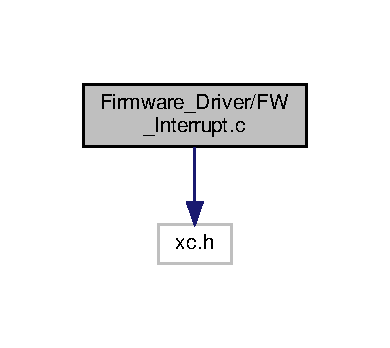
\includegraphics[width=187pt]{d1/d2f/FW__Interrupt_8c__incl}
\end{center}
\end{figure}
\subsection*{Funciones}
\begin{DoxyCompactItemize}
\item 
void \hyperlink{FW__Interrupt_8c_a9c2f60604071e2b4583e463e6825e708}{\+\_\+\+\_\+interrupt} ()
\begin{DoxyCompactList}\small\item\em Funcion de interrupcion. \end{DoxyCompactList}\end{DoxyCompactItemize}


\subsection{Documentación de las funciones}
\mbox{\Hypertarget{FW__Interrupt_8c_a9c2f60604071e2b4583e463e6825e708}\label{FW__Interrupt_8c_a9c2f60604071e2b4583e463e6825e708}} 
\index{F\+W\+\_\+\+Interrupt.\+c@{F\+W\+\_\+\+Interrupt.\+c}!\+\_\+\+\_\+interrupt@{\+\_\+\+\_\+interrupt}}
\index{\+\_\+\+\_\+interrupt@{\+\_\+\+\_\+interrupt}!F\+W\+\_\+\+Interrupt.\+c@{F\+W\+\_\+\+Interrupt.\+c}}
\subsubsection{\texorpdfstring{\+\_\+\+\_\+interrupt()}{\_\_interrupt()}}
{\footnotesize\ttfamily \+\_\+\+\_\+interrupt (\begin{DoxyParamCaption}{ }\end{DoxyParamCaption})}



Funcion de interrupcion. 

\begin{DoxyAuthor}{Autor}
Nicolas Ferragamo 
\end{DoxyAuthor}
\begin{DoxyDate}{Fecha}
23 de abril de 2019 
\end{DoxyDate}

\begin{DoxyParams}[1]{Parámetros}
\mbox{\tt in}  & {\em void} & \\
\hline
\mbox{\tt out}  & {\em void} & \\
\hline
\end{DoxyParams}
\begin{DoxyReturn}{Devuelve}
void 
\end{DoxyReturn}


Definición en la línea 70 del archivo F\+W\+\_\+\+Interrupt.\+c.


\hypertarget{FW__InitKit_8c}{}\section{Referencia del Archivo Firmware\+\_\+\+Init/\+F\+W\+\_\+\+Init\+Kit.c}
\label{FW__InitKit_8c}\index{Firmware\+\_\+\+Init/\+F\+W\+\_\+\+Init\+Kit.\+c@{Firmware\+\_\+\+Init/\+F\+W\+\_\+\+Init\+Kit.\+c}}
{\ttfamily \#include $<$xc.\+h$>$}\newline
{\ttfamily \#include \char`\"{}F\+W\+\_\+\+Init\+Kit.\+h\char`\"{}}\newline
Dependencia gráfica adjunta para F\+W\+\_\+\+Init\+Kit.\+c\+:
\nopagebreak
\begin{figure}[H]
\begin{center}
\leavevmode
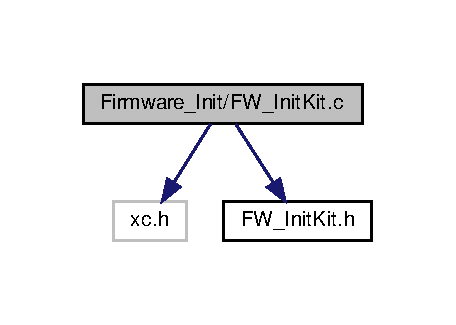
\includegraphics[width=219pt]{de/da1/FW__InitKit_8c__incl}
\end{center}
\end{figure}
\subsection*{Funciones}
\begin{DoxyCompactItemize}
\item 
void \hyperlink{FW__InitKit_8c_a91a9e93581be29c6af058d09741ee5be}{Kit\+\_\+\+Init} (void)
\begin{DoxyCompactList}\small\item\em Inicializa el entrenador. \end{DoxyCompactList}\end{DoxyCompactItemize}


\subsection{Documentación de las funciones}
\mbox{\Hypertarget{FW__InitKit_8c_a91a9e93581be29c6af058d09741ee5be}\label{FW__InitKit_8c_a91a9e93581be29c6af058d09741ee5be}} 
\index{F\+W\+\_\+\+Init\+Kit.\+c@{F\+W\+\_\+\+Init\+Kit.\+c}!Kit\+\_\+\+Init@{Kit\+\_\+\+Init}}
\index{Kit\+\_\+\+Init@{Kit\+\_\+\+Init}!F\+W\+\_\+\+Init\+Kit.\+c@{F\+W\+\_\+\+Init\+Kit.\+c}}
\subsubsection{\texorpdfstring{Kit\+\_\+\+Init()}{Kit\_Init()}}
{\footnotesize\ttfamily void Kit\+\_\+\+Init (\begin{DoxyParamCaption}\item[{void}]{ }\end{DoxyParamCaption})}



Inicializa el entrenador. 

Inicializa todos los puertos del entrenador preparandolo para usar el display y deshabilitando los comparadores de entrada y los canales anal�gicos. Tambi�n limpia todas las salidas. \begin{DoxyAuthor}{Autor}
Esteban Lemos 
\end{DoxyAuthor}
\begin{DoxyDate}{Fecha}

\end{DoxyDate}

\begin{DoxyParams}[1]{Parámetros}
\mbox{\tt in}  & {\em void} & \\
\hline
\mbox{\tt out}  & {\em void} & \\
\hline
\end{DoxyParams}
\begin{DoxyReturn}{Devuelve}
void 
\end{DoxyReturn}


Definición en la línea 64 del archivo F\+W\+\_\+\+Init\+Kit.\+c.

Gráfico de llamadas a esta función\+:
\nopagebreak
\begin{figure}[H]
\begin{center}
\leavevmode
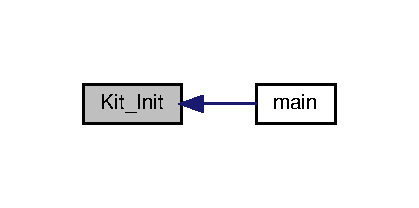
\includegraphics[width=201pt]{d6/d67/FW__InitKit_8c_a91a9e93581be29c6af058d09741ee5be_icgraph}
\end{center}
\end{figure}

\hypertarget{FW__InitTimer_8c}{}\section{Referencia del Archivo Firmware\+\_\+\+Init/\+F\+W\+\_\+\+Init\+Timer.c}
\label{FW__InitTimer_8c}\index{Firmware\+\_\+\+Init/\+F\+W\+\_\+\+Init\+Timer.\+c@{Firmware\+\_\+\+Init/\+F\+W\+\_\+\+Init\+Timer.\+c}}
{\ttfamily \#include \char`\"{}F\+W\+\_\+\+Init\+Timer.\+h\char`\"{}}\newline
Dependencia gráfica adjunta para F\+W\+\_\+\+Init\+Timer.\+c\+:
\nopagebreak
\begin{figure}[H]
\begin{center}
\leavevmode
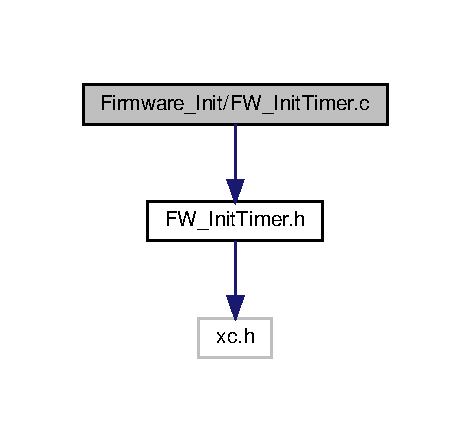
\includegraphics[width=226pt]{db/d06/FW__InitTimer_8c__incl}
\end{center}
\end{figure}
\subsection*{Funciones}
\begin{DoxyCompactItemize}
\item 
void \hyperlink{FW__InitTimer_8c_a9b69990a6c6d5341aafbd59794b6a7a3}{Tmr0\+\_\+\+Init} ()
\begin{DoxyCompactList}\small\item\em Inicializacion del Tmr0. \end{DoxyCompactList}\end{DoxyCompactItemize}


\subsection{Documentación de las funciones}
\mbox{\Hypertarget{FW__InitTimer_8c_a9b69990a6c6d5341aafbd59794b6a7a3}\label{FW__InitTimer_8c_a9b69990a6c6d5341aafbd59794b6a7a3}} 
\index{F\+W\+\_\+\+Init\+Timer.\+c@{F\+W\+\_\+\+Init\+Timer.\+c}!Tmr0\+\_\+\+Init@{Tmr0\+\_\+\+Init}}
\index{Tmr0\+\_\+\+Init@{Tmr0\+\_\+\+Init}!F\+W\+\_\+\+Init\+Timer.\+c@{F\+W\+\_\+\+Init\+Timer.\+c}}
\subsubsection{\texorpdfstring{Tmr0\+\_\+\+Init()}{Tmr0\_Init()}}
{\footnotesize\ttfamily Tmr0\+\_\+\+Init (\begin{DoxyParamCaption}\item[{void}]{ }\end{DoxyParamCaption})}



Inicializacion del Tmr0. 

Inicializa el timer 0 en 8 bits, con el prescaler en 256 y con la interrupcion activada. Esta configurado para que interrumpa cada 1.\+0022ms \begin{DoxyAuthor}{Autor}
I Esteban Lemos 
\end{DoxyAuthor}
\begin{DoxyDate}{Fecha}

\end{DoxyDate}

\begin{DoxyParams}[1]{Parámetros}
\mbox{\tt in}  & {\em void} & \\
\hline
\mbox{\tt out}  & {\em void} & \\
\hline
\end{DoxyParams}
\begin{DoxyReturn}{Devuelve}
void 
\end{DoxyReturn}


Definición en la línea 63 del archivo F\+W\+\_\+\+Init\+Timer.\+c.

Gráfico de llamadas a esta función\+:
\nopagebreak
\begin{figure}[H]
\begin{center}
\leavevmode
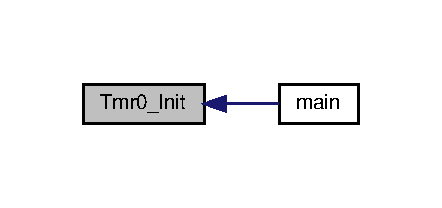
\includegraphics[width=212pt]{d2/d7e/FW__InitTimer_8c_a9b69990a6c6d5341aafbd59794b6a7a3_icgraph}
\end{center}
\end{figure}

\hypertarget{confbits_8h}{}\section{Referencia del Archivo inc/confbits.h}
\label{confbits_8h}\index{inc/confbits.\+h@{inc/confbits.\+h}}
Gráfico de los archivos que directa o indirectamente incluyen a este archivo\+:
\nopagebreak
\begin{figure}[H]
\begin{center}
\leavevmode
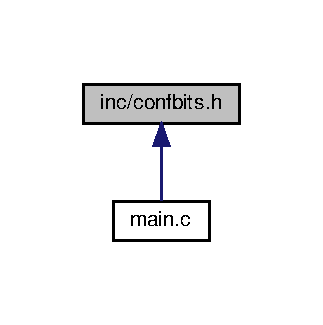
\includegraphics[width=155pt]{db/d61/confbits_8h__dep__incl}
\end{center}
\end{figure}

\hypertarget{FW__InitKit_8h}{}\section{Referencia del Archivo inc/\+F\+W\+\_\+\+Init\+Kit.h}
\label{FW__InitKit_8h}\index{inc/\+F\+W\+\_\+\+Init\+Kit.\+h@{inc/\+F\+W\+\_\+\+Init\+Kit.\+h}}
Gráfico de los archivos que directa o indirectamente incluyen a este archivo\+:
\nopagebreak
\begin{figure}[H]
\begin{center}
\leavevmode
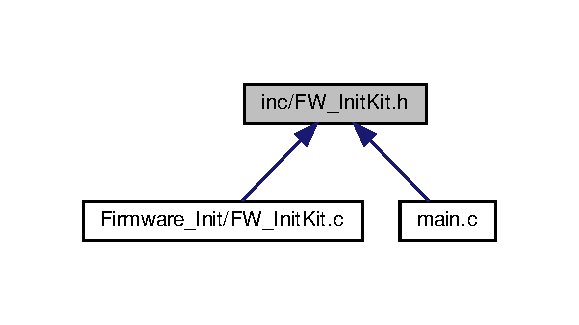
\includegraphics[width=278pt]{d5/d7d/FW__InitKit_8h__dep__incl}
\end{center}
\end{figure}
\subsection*{defines}
\begin{DoxyCompactItemize}
\item 
\#define \hyperlink{FW__InitKit_8h_aefae505e2588183f1921a9e840b16044}{L\+E\+D5}~L\+A\+T\+Dbits.\+L\+D0
\begin{DoxyCompactList}\small\item\em Indica ingreso a modo Boot\+Loader, puede ser usado por el usuario. \end{DoxyCompactList}\item 
\#define \hyperlink{FW__InitKit_8h_ab922b15d42b90025c9e13c087d86ce81}{L\+E\+D6}~L\+A\+T\+Dbits.\+L\+D1
\begin{DoxyCompactList}\small\item\em Inica modo conectado, puede ser usado por el usuario. \end{DoxyCompactList}\item 
\#define \hyperlink{FW__InitKit_8h_a8aa85ae9867fabf70ec72cd3bf6fb6b9}{L\+E\+D1}~L\+A\+T\+Dbits.\+L\+D2
\item 
\#define \hyperlink{FW__InitKit_8h_ad09fe5bf321b9a2de26bd5e5b9af6424}{L\+E\+D2}~L\+A\+T\+Dbits.\+L\+D3
\item 
\#define \hyperlink{FW__InitKit_8h_a4b7ff8e253a7412f83deba3a447028a8}{L\+E\+D3}~L\+A\+T\+Cbits.\+L\+C6
\item 
\#define \hyperlink{FW__InitKit_8h_ae048837f20072bed467332b1bd1da9fa}{L\+E\+D4}~L\+A\+T\+Cbits.\+L\+C7
\item 
\#define \hyperlink{FW__InitKit_8h_a514fed6fb5235478075a85e1a50b2aa7}{B\+O\+T1}~P\+O\+R\+T\+Dbits.\+R\+D4
\item 
\#define \hyperlink{FW__InitKit_8h_a9de2fc6886584e508307bc2e6a5ab6d6}{B\+O\+T2}~P\+O\+R\+T\+Dbits.\+R\+D5
\item 
\#define \hyperlink{FW__InitKit_8h_a145570f189e6e1523bf1dec991f477e7}{B\+O\+T3}~P\+O\+R\+T\+Dbits.\+R\+D6
\item 
\#define \hyperlink{FW__InitKit_8h_ac54405c71508dad19a53e9c85c1462ef}{B\+O\+T4}~P\+O\+R\+T\+Dbits.\+R\+D7
\item 
\#define \hyperlink{FW__InitKit_8h_a51ed185096fb63d11fe581879d4dd724}{D\+I\+S\+P1}~L\+A\+T\+Abits.\+L\+A4
\item 
\#define \hyperlink{FW__InitKit_8h_abfd463b3ac57b2cc718abf1e9f07ee9c}{D\+I\+S\+P2}~L\+A\+T\+Abits.\+L\+A5
\item 
\#define \hyperlink{FW__InitKit_8h_a6d6e11b0c9cc074a2c9af1747e68ef74}{D\+I\+S\+P3}~L\+A\+T\+Ebits.\+L\+E0
\item 
\#define \hyperlink{FW__InitKit_8h_ad0225737fa73024abb640898eed601df}{D\+I\+S\+P4}~L\+A\+T\+Ebits.\+L\+E1
\item 
\#define \hyperlink{FW__InitKit_8h_a8a5043e7ab655e37e903ffbd8b95d6b2}{D\+OT}~L\+A\+T\+Ebits.\+L\+E2
\end{DoxyCompactItemize}
\subsection*{Funciones}
\begin{DoxyCompactItemize}
\item 
void \hyperlink{FW__InitKit_8h_a91a9e93581be29c6af058d09741ee5be}{Kit\+\_\+\+Init} (void)
\begin{DoxyCompactList}\small\item\em Inicializa el entrenador. \end{DoxyCompactList}\end{DoxyCompactItemize}


\subsection{Documentación de los \textquotesingle{}defines\textquotesingle{}}
\mbox{\Hypertarget{FW__InitKit_8h_a514fed6fb5235478075a85e1a50b2aa7}\label{FW__InitKit_8h_a514fed6fb5235478075a85e1a50b2aa7}} 
\index{F\+W\+\_\+\+Init\+Kit.\+h@{F\+W\+\_\+\+Init\+Kit.\+h}!B\+O\+T1@{B\+O\+T1}}
\index{B\+O\+T1@{B\+O\+T1}!F\+W\+\_\+\+Init\+Kit.\+h@{F\+W\+\_\+\+Init\+Kit.\+h}}
\subsubsection{\texorpdfstring{B\+O\+T1}{BOT1}}
{\footnotesize\ttfamily \#define B\+O\+T1~P\+O\+R\+T\+Dbits.\+R\+D4}



Definición en la línea 39 del archivo F\+W\+\_\+\+Init\+Kit.\+h.

\mbox{\Hypertarget{FW__InitKit_8h_a9de2fc6886584e508307bc2e6a5ab6d6}\label{FW__InitKit_8h_a9de2fc6886584e508307bc2e6a5ab6d6}} 
\index{F\+W\+\_\+\+Init\+Kit.\+h@{F\+W\+\_\+\+Init\+Kit.\+h}!B\+O\+T2@{B\+O\+T2}}
\index{B\+O\+T2@{B\+O\+T2}!F\+W\+\_\+\+Init\+Kit.\+h@{F\+W\+\_\+\+Init\+Kit.\+h}}
\subsubsection{\texorpdfstring{B\+O\+T2}{BOT2}}
{\footnotesize\ttfamily \#define B\+O\+T2~P\+O\+R\+T\+Dbits.\+R\+D5}



Definición en la línea 40 del archivo F\+W\+\_\+\+Init\+Kit.\+h.

\mbox{\Hypertarget{FW__InitKit_8h_a145570f189e6e1523bf1dec991f477e7}\label{FW__InitKit_8h_a145570f189e6e1523bf1dec991f477e7}} 
\index{F\+W\+\_\+\+Init\+Kit.\+h@{F\+W\+\_\+\+Init\+Kit.\+h}!B\+O\+T3@{B\+O\+T3}}
\index{B\+O\+T3@{B\+O\+T3}!F\+W\+\_\+\+Init\+Kit.\+h@{F\+W\+\_\+\+Init\+Kit.\+h}}
\subsubsection{\texorpdfstring{B\+O\+T3}{BOT3}}
{\footnotesize\ttfamily \#define B\+O\+T3~P\+O\+R\+T\+Dbits.\+R\+D6}



Definición en la línea 41 del archivo F\+W\+\_\+\+Init\+Kit.\+h.

\mbox{\Hypertarget{FW__InitKit_8h_ac54405c71508dad19a53e9c85c1462ef}\label{FW__InitKit_8h_ac54405c71508dad19a53e9c85c1462ef}} 
\index{F\+W\+\_\+\+Init\+Kit.\+h@{F\+W\+\_\+\+Init\+Kit.\+h}!B\+O\+T4@{B\+O\+T4}}
\index{B\+O\+T4@{B\+O\+T4}!F\+W\+\_\+\+Init\+Kit.\+h@{F\+W\+\_\+\+Init\+Kit.\+h}}
\subsubsection{\texorpdfstring{B\+O\+T4}{BOT4}}
{\footnotesize\ttfamily \#define B\+O\+T4~P\+O\+R\+T\+Dbits.\+R\+D7}



Definición en la línea 42 del archivo F\+W\+\_\+\+Init\+Kit.\+h.

\mbox{\Hypertarget{FW__InitKit_8h_a51ed185096fb63d11fe581879d4dd724}\label{FW__InitKit_8h_a51ed185096fb63d11fe581879d4dd724}} 
\index{F\+W\+\_\+\+Init\+Kit.\+h@{F\+W\+\_\+\+Init\+Kit.\+h}!D\+I\+S\+P1@{D\+I\+S\+P1}}
\index{D\+I\+S\+P1@{D\+I\+S\+P1}!F\+W\+\_\+\+Init\+Kit.\+h@{F\+W\+\_\+\+Init\+Kit.\+h}}
\subsubsection{\texorpdfstring{D\+I\+S\+P1}{DISP1}}
{\footnotesize\ttfamily \#define D\+I\+S\+P1~L\+A\+T\+Abits.\+L\+A4}



Definición en la línea 44 del archivo F\+W\+\_\+\+Init\+Kit.\+h.

\mbox{\Hypertarget{FW__InitKit_8h_abfd463b3ac57b2cc718abf1e9f07ee9c}\label{FW__InitKit_8h_abfd463b3ac57b2cc718abf1e9f07ee9c}} 
\index{F\+W\+\_\+\+Init\+Kit.\+h@{F\+W\+\_\+\+Init\+Kit.\+h}!D\+I\+S\+P2@{D\+I\+S\+P2}}
\index{D\+I\+S\+P2@{D\+I\+S\+P2}!F\+W\+\_\+\+Init\+Kit.\+h@{F\+W\+\_\+\+Init\+Kit.\+h}}
\subsubsection{\texorpdfstring{D\+I\+S\+P2}{DISP2}}
{\footnotesize\ttfamily \#define D\+I\+S\+P2~L\+A\+T\+Abits.\+L\+A5}



Definición en la línea 45 del archivo F\+W\+\_\+\+Init\+Kit.\+h.

\mbox{\Hypertarget{FW__InitKit_8h_a6d6e11b0c9cc074a2c9af1747e68ef74}\label{FW__InitKit_8h_a6d6e11b0c9cc074a2c9af1747e68ef74}} 
\index{F\+W\+\_\+\+Init\+Kit.\+h@{F\+W\+\_\+\+Init\+Kit.\+h}!D\+I\+S\+P3@{D\+I\+S\+P3}}
\index{D\+I\+S\+P3@{D\+I\+S\+P3}!F\+W\+\_\+\+Init\+Kit.\+h@{F\+W\+\_\+\+Init\+Kit.\+h}}
\subsubsection{\texorpdfstring{D\+I\+S\+P3}{DISP3}}
{\footnotesize\ttfamily \#define D\+I\+S\+P3~L\+A\+T\+Ebits.\+L\+E0}



Definición en la línea 46 del archivo F\+W\+\_\+\+Init\+Kit.\+h.

\mbox{\Hypertarget{FW__InitKit_8h_ad0225737fa73024abb640898eed601df}\label{FW__InitKit_8h_ad0225737fa73024abb640898eed601df}} 
\index{F\+W\+\_\+\+Init\+Kit.\+h@{F\+W\+\_\+\+Init\+Kit.\+h}!D\+I\+S\+P4@{D\+I\+S\+P4}}
\index{D\+I\+S\+P4@{D\+I\+S\+P4}!F\+W\+\_\+\+Init\+Kit.\+h@{F\+W\+\_\+\+Init\+Kit.\+h}}
\subsubsection{\texorpdfstring{D\+I\+S\+P4}{DISP4}}
{\footnotesize\ttfamily \#define D\+I\+S\+P4~L\+A\+T\+Ebits.\+L\+E1}



Definición en la línea 47 del archivo F\+W\+\_\+\+Init\+Kit.\+h.

\mbox{\Hypertarget{FW__InitKit_8h_a8a5043e7ab655e37e903ffbd8b95d6b2}\label{FW__InitKit_8h_a8a5043e7ab655e37e903ffbd8b95d6b2}} 
\index{F\+W\+\_\+\+Init\+Kit.\+h@{F\+W\+\_\+\+Init\+Kit.\+h}!D\+OT@{D\+OT}}
\index{D\+OT@{D\+OT}!F\+W\+\_\+\+Init\+Kit.\+h@{F\+W\+\_\+\+Init\+Kit.\+h}}
\subsubsection{\texorpdfstring{D\+OT}{DOT}}
{\footnotesize\ttfamily \#define D\+OT~L\+A\+T\+Ebits.\+L\+E2}



Definición en la línea 48 del archivo F\+W\+\_\+\+Init\+Kit.\+h.

\mbox{\Hypertarget{FW__InitKit_8h_a8aa85ae9867fabf70ec72cd3bf6fb6b9}\label{FW__InitKit_8h_a8aa85ae9867fabf70ec72cd3bf6fb6b9}} 
\index{F\+W\+\_\+\+Init\+Kit.\+h@{F\+W\+\_\+\+Init\+Kit.\+h}!L\+E\+D1@{L\+E\+D1}}
\index{L\+E\+D1@{L\+E\+D1}!F\+W\+\_\+\+Init\+Kit.\+h@{F\+W\+\_\+\+Init\+Kit.\+h}}
\subsubsection{\texorpdfstring{L\+E\+D1}{LED1}}
{\footnotesize\ttfamily \#define L\+E\+D1~L\+A\+T\+Dbits.\+L\+D2}



Definición en la línea 34 del archivo F\+W\+\_\+\+Init\+Kit.\+h.

\mbox{\Hypertarget{FW__InitKit_8h_ad09fe5bf321b9a2de26bd5e5b9af6424}\label{FW__InitKit_8h_ad09fe5bf321b9a2de26bd5e5b9af6424}} 
\index{F\+W\+\_\+\+Init\+Kit.\+h@{F\+W\+\_\+\+Init\+Kit.\+h}!L\+E\+D2@{L\+E\+D2}}
\index{L\+E\+D2@{L\+E\+D2}!F\+W\+\_\+\+Init\+Kit.\+h@{F\+W\+\_\+\+Init\+Kit.\+h}}
\subsubsection{\texorpdfstring{L\+E\+D2}{LED2}}
{\footnotesize\ttfamily \#define L\+E\+D2~L\+A\+T\+Dbits.\+L\+D3}



Definición en la línea 35 del archivo F\+W\+\_\+\+Init\+Kit.\+h.

\mbox{\Hypertarget{FW__InitKit_8h_a4b7ff8e253a7412f83deba3a447028a8}\label{FW__InitKit_8h_a4b7ff8e253a7412f83deba3a447028a8}} 
\index{F\+W\+\_\+\+Init\+Kit.\+h@{F\+W\+\_\+\+Init\+Kit.\+h}!L\+E\+D3@{L\+E\+D3}}
\index{L\+E\+D3@{L\+E\+D3}!F\+W\+\_\+\+Init\+Kit.\+h@{F\+W\+\_\+\+Init\+Kit.\+h}}
\subsubsection{\texorpdfstring{L\+E\+D3}{LED3}}
{\footnotesize\ttfamily \#define L\+E\+D3~L\+A\+T\+Cbits.\+L\+C6}



Definición en la línea 36 del archivo F\+W\+\_\+\+Init\+Kit.\+h.

\mbox{\Hypertarget{FW__InitKit_8h_ae048837f20072bed467332b1bd1da9fa}\label{FW__InitKit_8h_ae048837f20072bed467332b1bd1da9fa}} 
\index{F\+W\+\_\+\+Init\+Kit.\+h@{F\+W\+\_\+\+Init\+Kit.\+h}!L\+E\+D4@{L\+E\+D4}}
\index{L\+E\+D4@{L\+E\+D4}!F\+W\+\_\+\+Init\+Kit.\+h@{F\+W\+\_\+\+Init\+Kit.\+h}}
\subsubsection{\texorpdfstring{L\+E\+D4}{LED4}}
{\footnotesize\ttfamily \#define L\+E\+D4~L\+A\+T\+Cbits.\+L\+C7}



Definición en la línea 37 del archivo F\+W\+\_\+\+Init\+Kit.\+h.

\mbox{\Hypertarget{FW__InitKit_8h_aefae505e2588183f1921a9e840b16044}\label{FW__InitKit_8h_aefae505e2588183f1921a9e840b16044}} 
\index{F\+W\+\_\+\+Init\+Kit.\+h@{F\+W\+\_\+\+Init\+Kit.\+h}!L\+E\+D5@{L\+E\+D5}}
\index{L\+E\+D5@{L\+E\+D5}!F\+W\+\_\+\+Init\+Kit.\+h@{F\+W\+\_\+\+Init\+Kit.\+h}}
\subsubsection{\texorpdfstring{L\+E\+D5}{LED5}}
{\footnotesize\ttfamily \#define L\+E\+D5~L\+A\+T\+Dbits.\+L\+D0}



Indica ingreso a modo Boot\+Loader, puede ser usado por el usuario. 



Definición en la línea 32 del archivo F\+W\+\_\+\+Init\+Kit.\+h.

\mbox{\Hypertarget{FW__InitKit_8h_ab922b15d42b90025c9e13c087d86ce81}\label{FW__InitKit_8h_ab922b15d42b90025c9e13c087d86ce81}} 
\index{F\+W\+\_\+\+Init\+Kit.\+h@{F\+W\+\_\+\+Init\+Kit.\+h}!L\+E\+D6@{L\+E\+D6}}
\index{L\+E\+D6@{L\+E\+D6}!F\+W\+\_\+\+Init\+Kit.\+h@{F\+W\+\_\+\+Init\+Kit.\+h}}
\subsubsection{\texorpdfstring{L\+E\+D6}{LED6}}
{\footnotesize\ttfamily \#define L\+E\+D6~L\+A\+T\+Dbits.\+L\+D1}



Inica modo conectado, puede ser usado por el usuario. 



Definición en la línea 33 del archivo F\+W\+\_\+\+Init\+Kit.\+h.



\subsection{Documentación de las funciones}
\mbox{\Hypertarget{FW__InitKit_8h_a91a9e93581be29c6af058d09741ee5be}\label{FW__InitKit_8h_a91a9e93581be29c6af058d09741ee5be}} 
\index{F\+W\+\_\+\+Init\+Kit.\+h@{F\+W\+\_\+\+Init\+Kit.\+h}!Kit\+\_\+\+Init@{Kit\+\_\+\+Init}}
\index{Kit\+\_\+\+Init@{Kit\+\_\+\+Init}!F\+W\+\_\+\+Init\+Kit.\+h@{F\+W\+\_\+\+Init\+Kit.\+h}}
\subsubsection{\texorpdfstring{Kit\+\_\+\+Init()}{Kit\_Init()}}
{\footnotesize\ttfamily void Kit\+\_\+\+Init (\begin{DoxyParamCaption}\item[{void}]{ }\end{DoxyParamCaption})}



Inicializa el entrenador. 

Inicializa todos los puertos del entrenador preparandolo para usar el display y deshabilitando los comparadores de entrada y los canales anal�gicos. Tambi�n limpia todas las salidas. \begin{DoxyAuthor}{Autor}
Esteban Lemos 
\end{DoxyAuthor}
\begin{DoxyDate}{Fecha}

\end{DoxyDate}

\begin{DoxyParams}[1]{Parámetros}
\mbox{\tt in}  & {\em void} & \\
\hline
\mbox{\tt out}  & {\em void} & \\
\hline
\end{DoxyParams}
\begin{DoxyReturn}{Devuelve}
void 
\end{DoxyReturn}


Definición en la línea 64 del archivo F\+W\+\_\+\+Init\+Kit.\+c.

Gráfico de llamadas a esta función\+:
\nopagebreak
\begin{figure}[H]
\begin{center}
\leavevmode
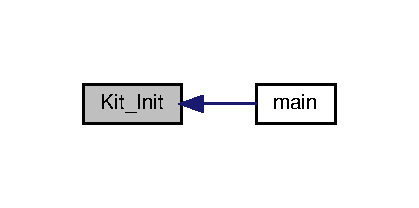
\includegraphics[width=201pt]{d5/dee/FW__InitKit_8h_a91a9e93581be29c6af058d09741ee5be_icgraph}
\end{center}
\end{figure}

\hypertarget{FW__InitTimer_8h}{}\section{Referencia del Archivo inc/\+F\+W\+\_\+\+Init\+Timer.h}
\label{FW__InitTimer_8h}\index{inc/\+F\+W\+\_\+\+Init\+Timer.\+h@{inc/\+F\+W\+\_\+\+Init\+Timer.\+h}}
{\ttfamily \#include $<$xc.\+h$>$}\newline
Dependencia gráfica adjunta para F\+W\+\_\+\+Init\+Timer.\+h\+:
\nopagebreak
\begin{figure}[H]
\begin{center}
\leavevmode
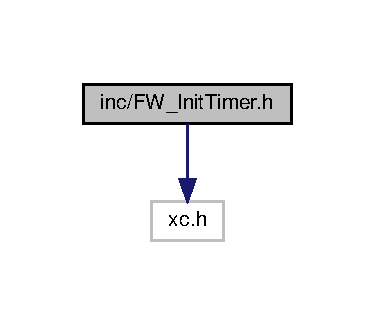
\includegraphics[width=180pt]{da/d12/FW__InitTimer_8h__incl}
\end{center}
\end{figure}
Gráfico de los archivos que directa o indirectamente incluyen a este archivo\+:
\nopagebreak
\begin{figure}[H]
\begin{center}
\leavevmode
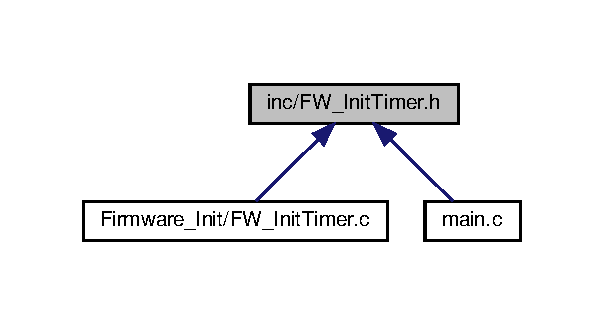
\includegraphics[width=290pt]{d0/d6f/FW__InitTimer_8h__dep__incl}
\end{center}
\end{figure}
\subsection*{Funciones}
\begin{DoxyCompactItemize}
\item 
void \hyperlink{FW__InitTimer_8h_abd382c7fbfb96997eaf343338a95fba1}{Tmr0\+\_\+\+Init} (void)
\begin{DoxyCompactList}\small\item\em Inicializacion del Tmr0. \end{DoxyCompactList}\end{DoxyCompactItemize}


\subsection{Documentación de las funciones}
\mbox{\Hypertarget{FW__InitTimer_8h_abd382c7fbfb96997eaf343338a95fba1}\label{FW__InitTimer_8h_abd382c7fbfb96997eaf343338a95fba1}} 
\index{F\+W\+\_\+\+Init\+Timer.\+h@{F\+W\+\_\+\+Init\+Timer.\+h}!Tmr0\+\_\+\+Init@{Tmr0\+\_\+\+Init}}
\index{Tmr0\+\_\+\+Init@{Tmr0\+\_\+\+Init}!F\+W\+\_\+\+Init\+Timer.\+h@{F\+W\+\_\+\+Init\+Timer.\+h}}
\subsubsection{\texorpdfstring{Tmr0\+\_\+\+Init()}{Tmr0\_Init()}}
{\footnotesize\ttfamily void Tmr0\+\_\+\+Init (\begin{DoxyParamCaption}\item[{void}]{ }\end{DoxyParamCaption})}



Inicializacion del Tmr0. 

Inicializa el timer 0 en 8 bits, con el prescaler en 256 y con la interrupcion activada. Esta configurado para que interrumpa cada 1.\+0022ms \begin{DoxyAuthor}{Autor}
I Esteban Lemos 
\end{DoxyAuthor}
\begin{DoxyDate}{Fecha}

\end{DoxyDate}

\begin{DoxyParams}[1]{Parámetros}
\mbox{\tt in}  & {\em void} & \\
\hline
\mbox{\tt out}  & {\em void} & \\
\hline
\end{DoxyParams}
\begin{DoxyReturn}{Devuelve}
void 
\end{DoxyReturn}


Definición en la línea 63 del archivo F\+W\+\_\+\+Init\+Timer.\+c.

Gráfico de llamadas a esta función\+:
\nopagebreak
\begin{figure}[H]
\begin{center}
\leavevmode
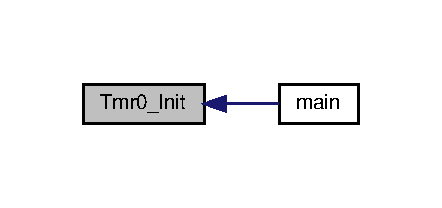
\includegraphics[width=212pt]{da/d62/FW__InitTimer_8h_abd382c7fbfb96997eaf343338a95fba1_icgraph}
\end{center}
\end{figure}

\hypertarget{main_8c}{}\section{Referencia del Archivo main.\+c}
\label{main_8c}\index{main.\+c@{main.\+c}}
{\ttfamily \#include $<$xc.\+h$>$}\newline
{\ttfamily \#include \char`\"{}confbits.\+h\char`\"{}}\newline
{\ttfamily \#include \char`\"{}F\+W\+\_\+\+Init\+Kit.\+h\char`\"{}}\newline
{\ttfamily \#include \char`\"{}F\+W\+\_\+\+Init\+Timer.\+h\char`\"{}}\newline
Dependencia gráfica adjunta para main.\+c\+:
\nopagebreak
\begin{figure}[H]
\begin{center}
\leavevmode
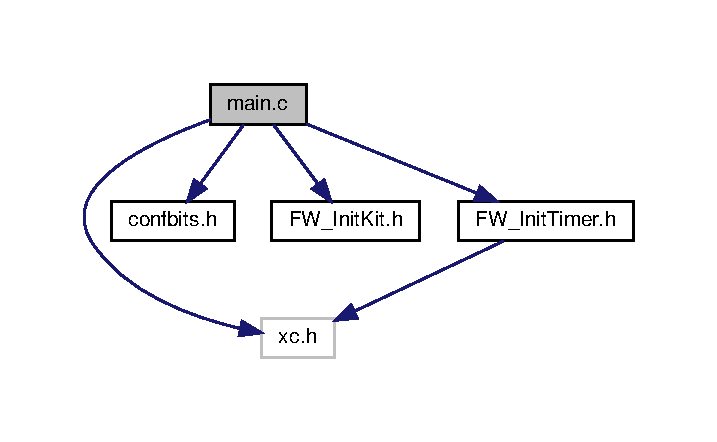
\includegraphics[width=344pt]{d4/d10/main_8c__incl}
\end{center}
\end{figure}
\subsection*{Funciones}
\begin{DoxyCompactItemize}
\item 
void \hyperlink{main_8c_a6288eba0f8e8ad3ab1544ad731eb7667}{main} (void)
\end{DoxyCompactItemize}


\subsection{Documentación de las funciones}
\mbox{\Hypertarget{main_8c_a6288eba0f8e8ad3ab1544ad731eb7667}\label{main_8c_a6288eba0f8e8ad3ab1544ad731eb7667}} 
\index{main.\+c@{main.\+c}!main@{main}}
\index{main@{main}!main.\+c@{main.\+c}}
\subsubsection{\texorpdfstring{main()}{main()}}
{\footnotesize\ttfamily void main (\begin{DoxyParamCaption}\item[{void}]{ }\end{DoxyParamCaption})}



Definición en la línea 60 del archivo main.\+c.


%--- End generated contents ---

% Index
\backmatter
\newpage
\phantomsection
\clearemptydoublepage
\addcontentsline{toc}{chapter}{Índice}
\printindex

\end{document}
